\pagebreak
\section{Motor Tests - Moment of Inertia} \label{app:motorTestMomentOfInertia}
\textbf{Name: Group 510}\\
\textbf{Date: 30/09 - 2015}

\subsubsection{Purpose}
The purpose of this test is to find the moment of inertia $I$, by measuring the motor velocity as a function of time.

\subsubsection{Setup}
\begin{figure}[H]
  \centering
	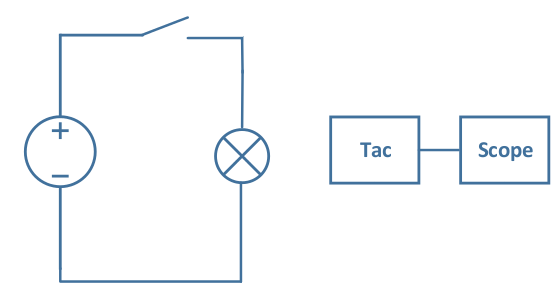
\includegraphics[scale=0.5]{figures/MotorTest8.png}
	\caption{Setup diagram}
\end{figure}
\todo{this figure does not make sense}

\subsubsection{List of Equipment}

\begin{table}[H]
\begin{tabular}{|l|l|p{4cm}|}
\hline%------------------------------------------------------------------------------------
  \textbf{Instrument}                        &  \textbf{AAU-no.}  &  \textbf{Type}       \\
\hline%------------------------------------------------------------------------------------
  Oscilloscope                               &  64672             &  Agilent DSO6034A    \\
\hline%------------------------------------------------------------------------------------
  Power Supply ($0 - 32$ V) ($0 - 10$ A)     &  77076             &  Ea - ps 7032 - 100  \\
\hline%------------------------------------------------------------------------------------
  Optical tachometer                         &  77087             &  Compact             \\
\hline%------------------------------------------------------------------------------------
\end{tabular}
\end{table}

\subsubsection{Procedure}

\begin{enumerate}
  \item Turn on the oscilloscope, and connect the tachometer to one of the inputs.
  \item On the oscilloscope press the "trigger mode"-key choose the "normal"-option, set the trigger to "falling edge".
  \item To prevent false triggering on the oscilloscope set the trigger value to \num{1,175} V with the turn-key.
  \item Turn on the power supply at 7 volt.
  \item Press "single"-key on oscilloscope and cut the power of the motor.
  \item Insert a USB-flash drive in the oscilloscope and press the save key to extract the data.
\end{enumerate}

\subsubsection{Results}

\begin{figure}[H]
  \setcounter{subfigure}{0}
  \centering
  \begin{subfigure}{0.48\textwidth}
    \centering
    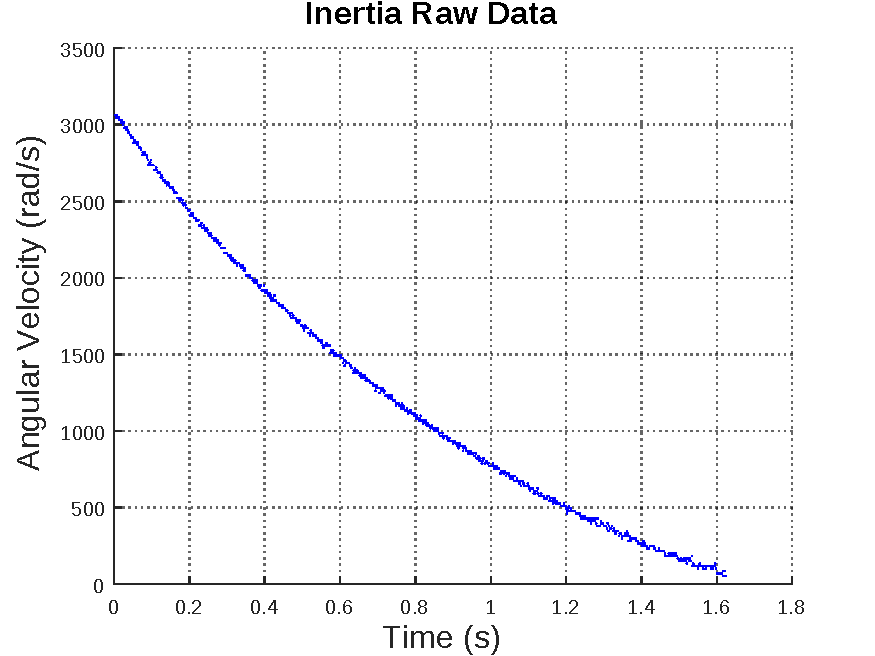
\includegraphics[width=1.2\linewidth]{figures/inertiaRawData.pdf}
    \caption{The measured angular velocity compared to time, where the blue line indicates the velocity after the power has been removed.}
    \label{inertiaRawData}
  \end{subfigure}
  \begin{subfigure}{0.48\textwidth}
    \centering
    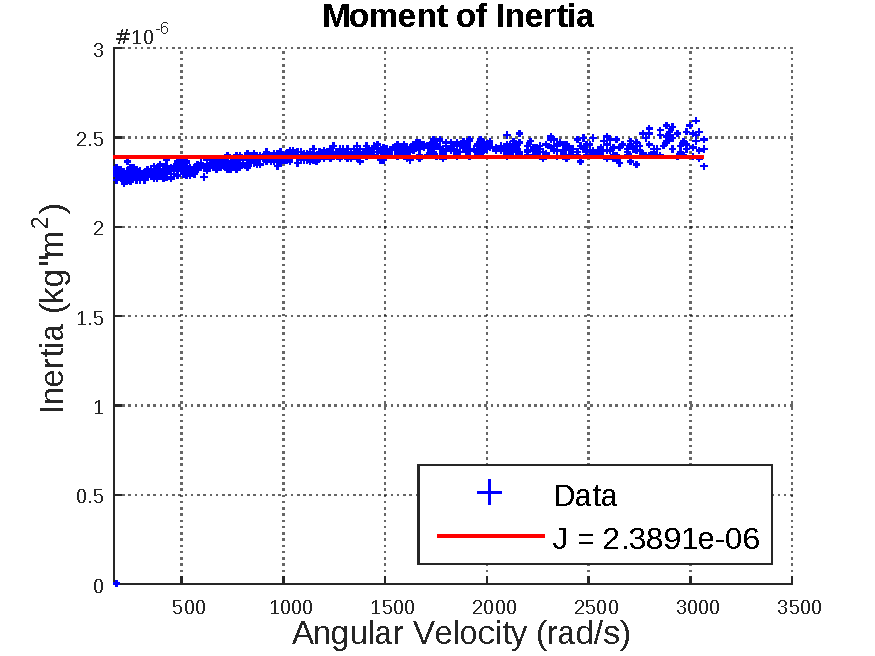
\includegraphics[width=1.2\linewidth]{figures/momentOfInertia.pdf}
    \caption{The Blue dots indicates the moment of inertia calculated using \eqref{eq:Momentofinertia}, and the red line represents the average value.}
  	\label{momentOfInertia}
  \end{subfigure}
  \caption{A plot of the inertia measured as the angular velocity compared to time and a plot of the moment of inertia calculated from the raw data using \eqref{eq:Momentofinertia}.}
  \label{yo}
\end{figure}

The equation used is given in the Modeling and Control course of the 5th semester on Electronic and IT at Aalborg University, \todo{reference}. This equation which arises from the mechanical description of the motor, when \si{i_a = 0} is used to find the Inertia, J.
\begin{flalign}
  \eq{\omega(s)}{- \frac{\tau_c}{B}+(\omega_0 + \frac{\tau_c}{B}) e^{-t\frac{B}{J}}}        \unit{rad\cdot s^{-1}}\nonumber\\
  &\Updownarrow&&\nonumber\\
  \eq{J}{ \frac{B\cdot t}{ln(  \frac{B\cdot \omega_0 + \tau_c}{B \cdot \omega + \tau_c})} } \unit{N\cdot m}
 \label{eq:Momentofinertia}
\end{flalign}

\hspace{6mm} Where:\\
\begin{tabular}{p{1cm}lll}
& \si{\omega(s)} & is the angular velocity        &\unitWh{rad \cdot s^{-1}}\\
& \si{\tau_c}    & is the coulomb friction torque &\unitWh{N \cdot m}     \\
& B              & is the friction                &\unitWh{N \cdot m}     \\
& J              & is the inertia                 &\unitWh{kg \cdot m^2}

\end{tabular}

The motor's inertia is calculated by using \eqref{eq:Momentofinertia} with the angular velocity compared to time illustrated on \figref{inertiaRawData}. Thereafter the average value of the results is found, seen in \figref{momentOfInertia} and used as the motor inertia. The motor's inertia is equal to:
%
\begin{flalign}
  \eq{J}{\num{2,3891} \cdot 10^{-6}}\ \si{kg \cdot m^2}&&\nonumber
\end{flalign}